\section{Plano de desenvolvimento pessoal de competências}
\qquad O meu plano de desenvolvimento pessoal, passa por obter mais formação e aprender com pessoas com mais experiência em diversas áreas, que é exatamente o que estou a fazer frequentando o curso de Engenharia Eletrotécnica e de Computadores no \textcolor{gray}{I.S.E.P}.\\
Esta disciplina em particular é uma forma de poder enriquecer minhas competências e metodologias de Gestão, e perceber as restantes matérias abordadas que compõem o \textcolor{blue}{Comportamento Organizacional}.\\
\begin{minipage}{8.5cm}
	\textbf{Metodologias da gestão}: \cite{book-9}
	\emptyline
	\begin{minipage}{3.1cm}
		Instrumental
		\begin{enumerate}
			\setlength\itemsep{-0.3em}
			\item Planear
			\item Organizar
			\item Controlar\\
		\end{enumerate}
	\end{minipage}
	\begin{minipage}{5cm}
		Comportamental
		\begin{enumerate}
			\setlength\itemsep{-0.3em}
			\item Liderança
			\item Comunicação
			\item Motivação
			\item Tomada de decisão
		\end{enumerate}
	\end{minipage}
\end{minipage}
\begin{minipage}{10cm}
\begin{figure}[H]
	\flushleft
	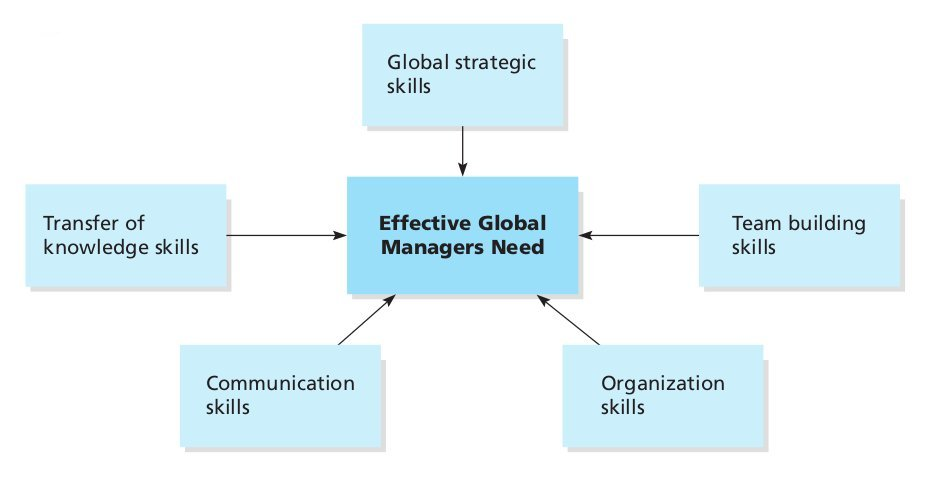
\includegraphics[scale=0.3]{./image/Skills/Managerial_Skills_for_the_Global_Marketplace.jpg}
	\caption{Competências de Gestão. \cite{book-6}}
\end{figure}
\end{minipage}
\emptyline
No entanto por enquanto minha missão é concluir a formação, e ao mesmo tempo melhorar um conjunto de ferramentas e métodos de trabalho para que seja estável e eficaz de forma a poder resolver os problemas que possa ter que enfrentar com facilidade, e eventualmente realizar alguns projetos pessoais.
\newpage
\subsection{Análise S.W.O.T Pessoal}
\qquad Neste contexto de plano de desenvolvimento a análise \textcolor{blue}{SWOT} também pode ser uma ferramenta útil de forma a nos indicar qual os comportamentos que poderá ser melhorado ou alterado.
\emptyline
\fbox{
\begin{minipage}[t]{\linewidth}
\begin{itemize}
	\setlength\itemsep{-0.85em}
	\item \textcolor{purple}{I}nterno
	\begin{itemize}
		\setlength\itemsep{-0.3em}
		\item \textcolor{orange}{S}trength (forças) \\
		- Numeração, Literacia Bilingue, Resolução de Problemas \\
		- Formação Académica, Experiência Profissional \\
		- Facilidade de Adaptação e aprendizagem, Imaginação \\
		- Gestão e Comunicação, Organização Pessoal \\
		- Numeração Avançada, Tecnologias de informação e comunicação. \\
		- Estabilidade Emocional \\
		- Empatia, Método Cientifico
		\item \textcolor{orange}{W}eakness (fraquezas) \\
		- Contabilidade e Vendas \\
		- Direto, Crítico, Detesto desigualdade e injustiças \\
		- Frontal com contradições \\
		- "Dente por dente e olho por olho" \\
		- Anti-Dogma
	\end{itemize}
	\item \textcolor{purple}{E}xterno
	\begin{itemize}
		\setlength\itemsep{-0.3em}
		\item \textcolor{orange}{O}pportunity (oportunidades) \\
		- Nenhum
		\item \textcolor{orange}{T}hreats (ameaças) \\
		- Cultura Portuguesa \\
		- Sistema Político-Social \\
		- Racismo
	\end{itemize}
\end{itemize}
\end{minipage}
}
\emptyline
Algumas explicações de personalidade descrevo no caso de quando se diz "dente por dente e olho por olho", muitas das vezes tem interpretação errada, pois concluem que existiria apenas cegos após alguns tempos, mas sendo uma metáfora, sabe-se que ninguém vai andar a cegar uns aos outros sem motivo e são circunstancias de saber individual, mas deve ser percebido no aspeto em que uma pessoa que é honesta merece honestidade, e uma humilde humildade, e pelo verso um mentiroso aldrabado, e assassino deve ser morto, este procedimento leva com que o bem vence sempre, isto é lógico e citações milenares de certa forma condiz neste caso. Que levanta também a questão da veracidade da perceção, na qual muito cuidado é exigido. \\
Dai que certas pessoas quando estão a ser irónicas, acabam dececionados com as reações esperadas, podendo entrar em ciclos viciosos que só vão agravando.
\emptyline
Quanto ao método cientifico nos diz que se um acontecimento se repete nas mesmas circunstâncias e nunca se altera é considerado facto ou lei ou teoria, é uma arte de reconhecer padrões. Também nós ensina que os conhecimentos estão sempre abertos ao escrutínio e se houver prova que refuta a teoria esta deixa de o ser, ou seja, é tentar representar a realidade observada por modelos racionais e matemáticos, as ferramentas que estão ao nosso dispor, já que não existe melhor.
\emptyline
Acho que esta análise seria mais prudente se fosse feito por uma perspetiva de terceiros, pois nos faria refletir nossas próprias preposições podendo ser reforçado ou até alterado.
\subsection{Curriculum Vitae}
\qquad Curriculum vitae significa "percurso de vida" \; em latim, ao primeiro era pouco conhecido e pouco utilizado, ou reservado apenas a uma fração da população ativa, principalmente aos jovens diplomados ou aos quadros que mudavam de "situação". No entanto os tempos mudaram devido a instabilidade e mudanças que levou a grande procura de novos empregos com muitos candidatos e o principal documento que terá os elementos fundamentais, que conduzem à apreciação e seleção é, sem dúvida, o CV.\cite{book-12}
O CV é um meio que permite a comunicação, para transmitir tua experiência profissional, tua personalidade na qual deve mencionar tuas motivações e objetivos algo que poderá separar dos restantes candidatos. \\
O Papel do CV serve para sermos selecionados para uma eventual entrevistas de trabalho, e consequentemente obter um acordo ou contrato de trabalho. Este documento é sempre um anexo nas candidaturas por qualquer via de comunicação, seja por e-mail ou contacto direto. \\
O CV em princípio deve conter tua identificação, morada, formação académica e literária, personalidade, experiência profissional e outros assuntos relacionados, ou seja, acaba por ser uma forma de divulgar as tuas competências de forma ordenada e organizada, para ser apelativo deve ser percetível e suscito, na qual só uma observação rápido pode ter uma ideia geral do candidato.
\emptyline
\textit{Anexado CV}.
